Gran parte del corso è dedicata allo studio dei diversi tipi di rivelatore, e per capire come funziona un rivelatore bisogna innanzitutto capire come la radiazione che vogliamo andare a rivelare interagisce con la materia, in quanto i rivelatori sfruttano proprio tali meccanismi di interazione per estrarre le informazioni utili per l'utente.

Cominceremo con una breve introduzione sui tipi di radiazione.

\section{Tipi di radiazione}

\subsection{Radiazioni ionizzanti}
Per ionizzante intendiamo qualcosa che riesce a innescare un fenomeno di ionizzazione nella materia, cioè riesce a creare una coppia ione-elettrone, quindi si strappa un elettrone all'atomo inizialmente neutro e si crea tale coppia. Tale fenomeno è detto \textit{ionizzazione}. Quando parliamo di radiazioni ionizzanti, intendiamo delle radiazioni che hanno energia tale da produrre effetto di ionizzazione o di un atomo o di una molecola. Esse possono essere di origine corpuscolare o elettromagnetica. In particolare sono:

\begin{itemize}
    \item Particelle subatomiche, quali elettroni e protoni. I neutroni sono un po' un caso a parte perché possono produrre effetti di ionizzazione attraverso altri meccanismi, ad esempio a seguito dell'interazione producono particelle cariche. Oltre a queste esiste uno zoo di particelle che, sebbene non esista in natura, può essere prodotto attraverso reazioni o collisioni; tra queste vi è il muone, che rappresenta una radiazione naturale in quanto è una parte della componente secondaria dei raggi cosmici.
    
    In generale quindi tutte le particelle cariche subatomiche, purché abbiano energia sufficiente per farlo, sono in grado di ionizzare la materia;
    \item Radiazioni elettromagnetiche con energia sufficiente. Infatti, lo spettro delle onde elettromagnetiche è molto vasto e si caratterizza in base alla frequenza dell'onda, da cui dipende l'energia della radiazione e quindi la capacità di ionizzare (ricordiamo che per ionizzare un atomo o una molecola è necessaria un'energia minima di ionizzazione, per cui ad esempio la luce visibile o le onde radio non riescono, mentre X, $\gamma$ sì).
\end{itemize}

\subsection{Sorgenti di radiazioni naturali}

\begin{itemize}
    \item Materiali emettitori naturali (ad esempio il Radon);
    \item Sorgenti radioattive (ad esempio isotopi radioattivi);
    \item Radiazione cosmica, che proviene dal cosmo, perché prodotta da sorgenti di origine astrofisica. In particolar modo noi non siamo sottoposti alla radiazione prodotte da tali sorgenti (che prende il nome di radiazione primaria), bensì alla radiazione secondaria, in quanto quella primaria quando incontra le molecole dell'atmosfera terrestre interagisce, producendo degli sciami di particelle secondarie. L'atmosfera dunque agisce da filtro, proteggendoci dalla radiazione primaria
\end{itemize}

Noi conviviamo con il livello di radiazione proveniente sia dagli isotopi naturali presenti nei materiali da costruzione, negli alimenti ecc. che dalla radiazione cosmica. Il nostro organismo si è quindi sviluppato in maniera tale da poter tollerare un certo livello di radiazione senza sviluppare dei danni di tipo biologico.

\subsection{Sorgenti di radiazioni artificiali}

\begin{itemize}
    \item Macchine acceleratrici per scopi o diagnostici (TAC, PET) con cui veniamo sottoposti a radiazioni prodotte da tali macchine, o terapeutici come la radioterapia con cui si è soggetti a radiazioni prodotte da isotopi iniettatici nell'organismo;
    \item Acceleratori di particelle, cioè strumenti in grado di generare fasci di particelle che possiedono una determinata energia.
\end{itemize}

\subsection{Radiazioni cariche}
Si tratta di particelle dotate di carica, che si distinguono in

\begin{itemize}
    \item Particelle cariche pesanti (protoni, alfa, ioni pesanti);
    \item Elettroni.
\end{itemize}

Tale distinzione viene fatta perché i meccanismi con cui le particelle cariche pesanti interagiscono con la materia sono diversi da quelli con cui interagiscono gli elettroni.

Ricordiamo che la massa elettrone è pari a $0.511 \; \rm MeV$ mentre la massa del protone è dell'ordine del $\rm GeV$, dunque tra i due c'è un fattore $2 \cdot 10^3$.

\subsection{Radiazioni neutre}
Associate a particelle neutre o a radiazione elettromagnetica:

\begin{itemize}
    \item Radiazione elettromagnetica (noi ci interesseremo di X e $\gamma$);
    \item Neutroni, ma non ci occuperemo molto di questi perché i loro meccanismi di interazione possono dar luogo a processi nucleari e formazione di particelle cariche, quindi producono ionizzazione attraverso meccanismi secondari.
\end{itemize}

\subsection{Radiazione cosmica secondaria}
Essa è una radiazione innescata dall'interazione dei cosmici primari con l'atmosfera. Sono costituiti principalmente da:

\begin{itemize}
    \item Muoni, il "cugino pesante dell'elettrone". \E una particella elementare come l'elettrone, ma con una massa di 200 volte circa quella dell'elettrone e può avere carica sia positiva che negativa ($\mu^{+}$ e $\mu^{-}$). Sono una particella molto penetrante, cioè riesce ad attraversare i vari strati dell'atmosfera giungendo fino al livello del mare (se ha energia sufficiente), costituendo la maggior parte delle radiazioni cosmiche secondarie. Hanno una vita media di pochi microsecondi, tuttavia riusciamo ad osservarle a terra per effetti relativistici (dilatazione del tempo). È difficile schermarsi dai muoni, per cui bisogna ricordarsi che un qualunque rivelatore li misurerà, quindi per esperimenti in cui essi rappresentano un rumore di fondo (perché interessati ad altri fenomeni) si lavora in caverne (ad esempio il laboratorio nazionale del Gran Sasso).
    \item Elettroni.
\end{itemize}

\section{Energia e potere penetrante}

\subsection{Range energia di interesse}

\begin{itemize}
    \item Sorgenti radioattive: da pochi $\rm eV$ (quindi poco energetiche) a $\rm 10^7 \; eV(=10MeV)$;
    \item Radiazione cosmica secondaria: dal $\rm MeV$ al $\rm GeV$. In questo caso le energie sono più alte perché in partenza i cosmici primari hanno delle energie notevoli (che non riusciamo a riprodurre con nessun acceleratore di particelle, tant'è che costituiscono l'accelerazione più grande che l'uomo abbia mai osservato) e di conseguenza anche i cosmici secondari.
\end{itemize}

\subsection{Capacità penetrazione radiazioni}

Indica quanto materiale le radiazioni riescono ad attraversare prima di essere arrestate. Si parla infatti di \textit{potere penetrante}.

\begin{itemize}
    \item Elettroni emessi da sorgenti radioattive ($\beta$): alcuni millimetri di materiale (hanno pochi $\rm MeV$);
    \item Particelle $\alpha$ da sorgenti: qualche centinaio di $\mu m$ di materiale solido, quindi rispetto alle particelle $\beta$ hanno meno potere penetrante in quanto, essendo particelle più pesanti (ricordiamo che sono nuclei di elio), nell'attraversamento perdono più facilmente la loro energia, arrestandosi in pochissimo spazio. Ad esempio nell'aria percorrono qualche centimetro.
    
    Sebbene ciò rappresenti un vantaggio dal punto di vista della radio-protezione, da quello della rivelazione delle particelle $\alpha$ rappresenta un problema perché rischiamo che i rivelatori non misurino niente in quanto le particelle vengono arrestate totalmente da pochi centimetri d'aria. Per questo motivo per tali radiazioni si adopera una camera da vuoto;
    \item Muoni cosmici: sono estremamente penetranti, per cui servono spessori anche di centinaia di metri per poter arrestare i muoni più energetici.
\end{itemize}

\section{Nuclei instabili}

Quando parliamo di sorgenti radioattive, intendiamo degli isotopi che decadono nel tempo, che sono quindi instabili, cioè cambiano la loro natura.

\begin{figure}[H]
    \centering
    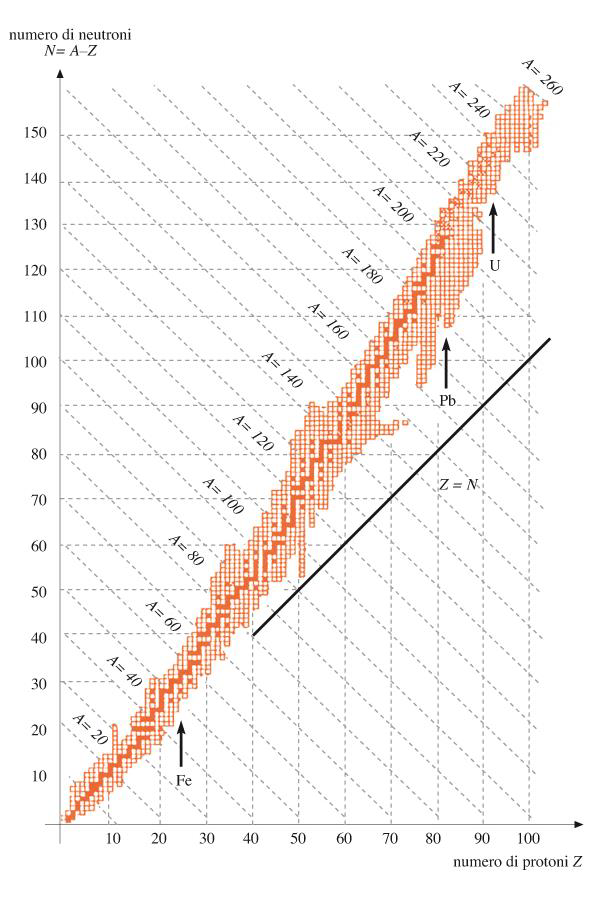
\includegraphics[width=9cm]{immagini/carta_di_segre.png}
\end{figure}

Nel grafico abbiamo il numero di protoni di un nucleo sulle ascisse ed il numero di neutroni sulle ordinate (rispettivamente $Z$ è il numero di protoni ed $N=A-Z$ il numero di neutroni).

La linea retta rappresenta la bisettrice del grafico. Se un nucleo si trova all'interno di essa allora avrà numero di protoni uguale al numero di neutroni.

In natura gli isotopi tendono a disporsi secondo la distribuzione arancione; in particolare i punti più scuri rappresentano gli isotopi stabili, che non decadono nel tempo e quindi non cambiano natura. Si osserva che la stabilità all'inizio, per i nuclei più leggeri, viene assicurata quando il nucleo possiede ugual numero di protoni e di neutroni (pensiamo ad esempio al $\rm C^{12}$, che ha 6 protoni e 6 neutroni). Ciò vale fino a $Z=20$; quando invece il numero di protoni aumenta e quindi il nucleo diventa più pesante, la condizione di stabilità si può avere solo quando il numero di neutroni è maggiore del numero di protoni. Il motivo è che, a causa della repulsione coulombiana tra i protoni che costituiscono il nucleo, è necessario un maggior numero di neutroni che fungono da "collante" grazie all'interazione forte.

Osservando il grafico notiamo che per ogni nucleo, cioè fissato un valore di $Z$, abbiamo, oltre al punto scuro, altri punti più chiari lungo la verticale che rappresentano tutti i possibili isotopi di un determinato nucleo al variare del numero di neutroni $N$. Ad esempio per l'idrogeno abbiamo il deuterio (due neutroni) e il trizio (tre neutroni), per il carbonio esiste il $\rm ^{13}C$ ed il $\rm ^{14}C$. Il fatto che siano colorati più chiari indica che sono instabili, cioè tendono a cambiare la loro natura nel tempo.

L'ultimo isotopo stabile che si trova in natura è il piombo, che ha $Z=82$; tutti gli isotopi più pesanti di esso sono instabili.

\section{Legge del decadimento radioattivo}

Tale legge è valida per tutti i decadimenti radioattivi. Essa ci dice che in un campione di $N$ isotopi instabili, il numero medio di nuclei che decade in un intervallo infinitesimo di tempo $\dd{t}$ è

\begin{equation*}
    \dd{N}=-\lambda N\dd{t}
\end{equation*}

Il numero infinitesimo $\dd{n}$ dipenderà quindi

\begin{itemize}
    \item Dal numero $N$ di isotopi di partenza;
    \item Dall'intervallo infinitesimo $\dd{t}$ considerato;
    \item Dalla costante $\lambda$ detta \textbf{costante di decadimento}, che è caratteristica di ciascun isotopo. Essa esprime la probabilità che il nucleo decada, quindi più è grande più nuclei decadono.
\end{itemize}

Il segno meno è dovuto al fatto che se i nuclei decadono il numero $N$ diminuisce.

Tale legge è un'equazione differenziale che ha come soluzione la vera e propria legge di decadimento radioattivo:

\begin{equation*}
    N(t)=N_0\,e^{-\lambda t}
\end{equation*}

dove $N_0$ è il numero iniziale di nuclei. Tale legge ci dice che il numero di nuclei ancora presenti nel campione all'istante generico $t$.

Talvolta anziché $\lambda$ si adopera una di queste due grandezze:

\begin{itemize}
    \item \textit{Vita media}: $\displaystyle \tau=\frac{1}{\lambda}$;
    \item \textit{Tempo di dimezzamento} o \textit{emivita}: $\displaystyle T_{\frac{1}{2}}=\frac{\ln{2}}{\lambda}$.
\end{itemize}

Entrambe le grandezze hanno le dimensioni di un tempo, dunque si misurano in secondi. In particolare la vita media corrisponde al tempo necessario affinché il numero di nuclei si riduca di un fattore $e$, cioè il tempo per passare da $N_0$ a $N_0/e$, l'emivita invece corrisponde al tempo necessario affinché il numero di nuclei di partenza si dimezzi, cioè il tempo per passare da $N_0$ a $N_0/2$. La relazione con la costante di decadimento si ricava tramite semplici passaggi matematici: imponendo $N(t)=N_0/2$ si ha che

\begin{equation*}
    \frac{N_0}{2}=N_0\,e^{-\lambda t}
    \implies
    -\ln{2}=-\lambda t
    \implies
    t=\frac{\ln{2}}{\lambda}
\end{equation*}

Le emivite variano da alcuni giorni a diversi miliardi di anni.

$T_{\frac{1}{2}}$ e $\tau$ sono legati tramite la relazione

\begin{equation*}
    T_{\frac{1}{2}}=\frac{\ln{2}}{\lambda}=\tau \ln{2}
\end{equation*}

Solitamente come riferimento per il tempo si prendono multipli dell'emivita perché è facile calcolare il corrispondente numero di isotopi restanti.

\begin{figure}[H]
    \centering
    \begin{tikzpicture}[xscale=1.6,yscale=1.3]
      \draw[->] (0,0) -- (5,0) node[right] {$t$};
      \draw[->] (0,0) -- (0,3.5) node[above] {$N$};
      %punti
      %punto iniziale
      \draw (0,3) -- (-0.1,3) node[left] {\footnotesize$N_0$};
      %dimezzamento
      \draw (0,1.5) -- (-0.1,1.5) node[left] {\footnotesize$N_0/2$};
      \draw[dashed] (0,1.5) -- (0.693,1.5) -- (0.693,0) node[below] {\footnotesize$T_{\frac{1}{2}}$};
      %fattore e
      \draw (0,1.104) -- (-0.1,1.104) node[left] {\footnotesize$N_0/e$};
      \draw[dashed] (0,1.104) -- (1,1.104) -- (1,0) node[below] {\footnotesize$\tau$};
      %un quarto
      \draw (0,0.75) -- (-0.1,0.75) node[left] {\footnotesize$N_0/4$};
      \draw[dashed] (0,0.75) -- (1.386,0.75) -- (1.386,0) node[below] {\footnotesize$2T_{\frac{1}{2}}$};
      %un ottavo
      \draw (0,0.375) -- (-0.1,0.375) node[left] {\footnotesize$N_0/8$};
      \draw[dashed] (0,0.375) -- (2.079,0.375) -- (2.079,0) node[below] {\footnotesize$3T_{\frac{1}{2}}$};
      %funzione
      \draw[thick, teal] plot[smooth, domain=0:4.5] (\x,{3*exp(-\x)});
    \end{tikzpicture}
  \end{figure}

%\begin{figure}[H]
%    \centering
%    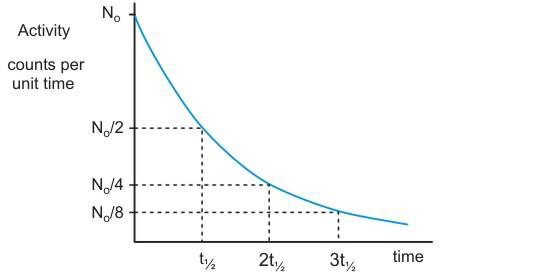
\includegraphics[width=12cm]{immagini/legge_decadimento_radioattivo_1.png}
%\end{figure}

Notiamo inoltre che il tempo di dimezzamento viene prima della vita media (del resto $\ln 2 < 1$). Infatti per $t=\tau$ si ha

$$N=N_0 \cdot e^{-\lambda \cdot \frac{1}{\lambda}}
=N_0 \cdot e^{-1}=\frac{N_0}{e}<\frac{N_0}{2}$$



Vediamo ora cosa cambia al variare del valore della costante di decadimento $\lambda$:

\begin{figure}[H]
    \centering
    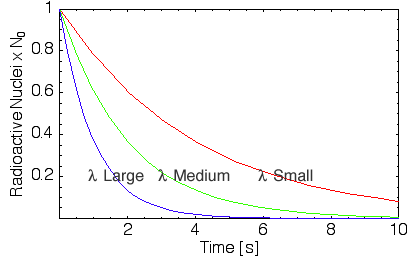
\includegraphics[width=11cm]{immagini/legge_decadimento_radioattivo_2.png}
\end{figure}

Se $\lambda$ è elevata, l'esponenziale è più rapido, cioè la probabilità di decadere è maggiore, per cui si dice che la sorgente ha un'elevata attività; viceversa, ad un valore piccolo di $\lambda$ corrisponde minore pendenza.

In termini di radioprotezione, $\lambda$ influisce anche sul tempo che deve trascorrere affinché il livello di radiazione emesso dal materiale non sia più dannoso per le persone.

Facciamo degli esempi con l'emivita (che è più facile da immaginare concettuamente) anziché la costante di decadimento:


\begin{center}
    \begin{tabular}{|l|l|}
        \hline
        Elemento & $T_{1/2}$\\
        \hline
        Radon 222 & 3.8 giorni\\
        \hline
        Piombo 210 & 22 anni\\
        \hline
        Radio 226 & 1600 anni\\
        \hline
        Carbonio 14 & 5730 anni\\
        \hline
        Uranio 238 & $4.56 \cdot 10^9$ anni\\
        \hline
    \end{tabular}
\end{center}

Notiamo come ci sia un'estrema variabilità nel valore del tempo di dimezzamento, quindi ci sono enormi differenze da isotopo a isotopo.

\subsection[Excursus: la datazione al carbonio \texorpdfstring{$\rm ^{14}C$}{\textonesuperior\textfoursuperior C}]
{Excursus: la datazione al carbonio $\boldsymbol{\rm ^{14}C}$}

L'isotopo $\rm ^{14}C$ ha un'emivita di 5730 anni. Esso viene usato per tecniche di datazione, cioè per sapere qual è l'età di un reperto di origine organica (ad esempio resti umani). Gli esseri viventi scambiano carbonio con l'atmosfera, ma con la morte dell'organismo tale scambio termina, e il $\rm ^{14}C$ presente nell'individuo (che fino ad ora si è tenuto costante grazie a tale scambio continuo) incomincia a decadere. Andando a vedere il quantitativo residuo di $\rm ^{14}C$ presente nell'organismo si può risalire, grazie alla legge di decadimento, all'età del campione.

Tale metodo non è utilizzabile con reperti eccessivamente antichi: la regola di norma è che al massimo possiamo datare campioni eventi età pari a 10 volte l'emivita del campione considerato, quindi al massimo 60 mila anni. Il motivo è che dopo 10 emivite il quantitativo di $\rm ^{14}C$ residuo è veramente poco, per cui non ci permette, da un punto di vista statistico, di fare una misura precisa dell'età del campione.

%\newpage

\section[Isotopi radioattivi \texorpdfstring{$\beta$}{\textbeta}]
{Isotopi radioattivi $\boldsymbol{\beta}$}

Il decadimento $\beta$ corrisponde all'emissione di elettroni o di positroni (rispettivamente decadimento $\beta^-$ e $\beta^+$). Ciò corrisponde rispettivamente alla trasformazione, all'interno del nucleo, di un neutrone in un protone, con l'emissione di un elettrone e di un antineuntrino elettronico, oppure viceversa alla trasformazione di un protone in un neutrone, con l'emissione di un positrone e di un neutrino elettronico:

\vspace{-0.3cm}

\begin{minipage}{0.395\textwidth}
    \begin{figure}[H]
        \centering
        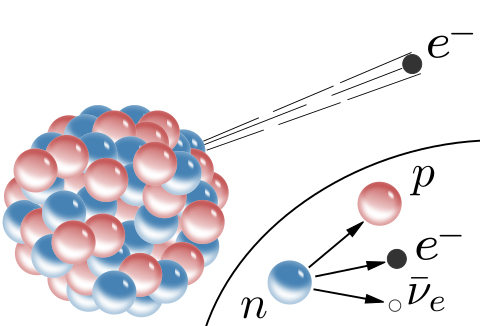
\includegraphics[width=5cm]{immagini/decadimento_beta.png}
    \end{figure}
\end{minipage}
\begin{minipage}{0.6\textwidth}
    \begin{center}
        \begin{tabular}{ll}
            $\beta^-: n \ce{->} p + e^- + $ & $(A,Z) \ce{ -> } (A,Z +1)$\\
            $\beta^+: p \ce{->} n + e^+ + \nu$ & $(A,Z) \ce{-> } (A,Z -1)$
        \end{tabular}
    \end{center}
\end{minipage}

\vspace{0.4cm}

Quando inizialmente si scoprì tale fenomeno, non si capiva se, oltre all'elettrone, venisse emesso un altro tipo di radiazione. Inoltre non si capiva l'origine di questi elettroni, perché le energie che si misuravano per queste particelle erano elevate, arrivavano all'ordine del MeV, cosa che fece capire che non potevano essere elettroni atomici, i quali non possono possedere tali energie. Si capì poi che erano elettroni provenienti dal nucleo.

Un'altra difficoltà che si ebbe riguardava l'energia di tali elettroni, in quanto non erano fisse: potevano variare tra un minimo e un massimo, cosa strana se l'unica particella emessa fosse stata l'elettrone, perché in tal caso allo stato finale avremmo avuto due corpi: il nucleo residuo e l'elettrone emesso, per cui se il nucleo a causa delle sue dimensioni assorbe pochissima energia questa sarebbe andata tutta all'elettrone, ma allora l'energia avrebbe dovuto avere un valore fisso. Ciò non si capiva perché i rivelatori dell'epoca misuravano solo l'emissione di elettroni. La spiegazione fu data dalla scoperta del fatto che viene emesso anche un neutrino, il quale è difficile da essere rivelato a causa della sua bassa sezione d'urto.

\vspace{0.4cm}

\begin{minipage}{0.345\textwidth}
    \vspace{-0.6cm}
    \begin{figure}[H]
        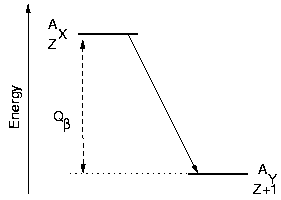
\includegraphics[width=5cm]{immagini/Isotopi_beta.png}
    \end{figure}
\end{minipage}
\begin{minipage}{0.65\textwidth}
    Dal punto di vista del nucleo, se esso ha numero di massa $A$ e numero atomico $Z$, dopo il decadimento avremo un nucleo residuo con stesso numero di massa ma numero atomico aumentato o diminuito di una unità a seconda del tipo di decadimento.

    Nella figura accanto possiamo vedere lo schema del decadimento nucleare di un nucleo $(A,Z)$ ad un nucleo $(A,Z+1)$. In questo caso si avrà l'emissione di un $\beta^-$.
\end{minipage}

\vspace{0.4cm}Questo decadimento avviene grazie ad un bilancio energetico che favorisce il nucleo finale.

Vediamo alcuni esempi di isotopi che decadono $\beta$:

\begin{center}
    \begin{tabular}{|l|l|l|}
        \hline
        Isotopo & Vita media & Energia massima (MeV)\\
        \hline
        &&\\[-0.45cm]
        $\rm ^3H$ & 12.26 y & 0.0186\\
        \hline
        &&\\[-0.45cm]
        $\rm ^{14}C$ & 5730 y & 0.156\\
        \hline
        &&\\[-0.45cm]
        $\rm ^{90}Sr / ^{90}Y$ & 27.7 y/64 h & 0.546/2.27\\
        \hline
        &&\\[-0.45cm]
        $\rm ^{99}Tc$ & $2.12 \cdot 10^5$ y & 0.292\\
        \hline
    \end{tabular}
\end{center}


In laboratorio adopereremo \ce{^{90}Sr} e \ce{^{90}Y} come sorgenti di raggi $\beta$.

\vspace{0.2cm}Il decadimento $\beta$ è a tre corpi (nucleo residuo, elettrone/positrone e neutrino), per cui l'energia si deve suddividere tra questi. Il nucleo residuo, essendo molto massivo, non acquisisce praticamente nulla, per cui il \textit{Q-value} di questo decadimento (cioè l'energia totale emessa nel decadimento) sì ripartisce tra l'elettrone e il neutrino, che sono gli elementi più leggeri; a seconda di come si suddividono l'energia, l'energia dell'elettrone varierà. In generale lo spettro delle energie ha forma come nel grafico: parte da un valore, sale fino a un massimo e poi scende, raggiungendo un massimo di energia detto \textit{endpoint dello spettro}. Nota: il punto iniziale è il valore minimo di energia perché sulle ascisse c'è l'energia.

\begin{minipage}{0.42\textwidth}
   \vspace{-0.9cm}\begin{figure}[H]
       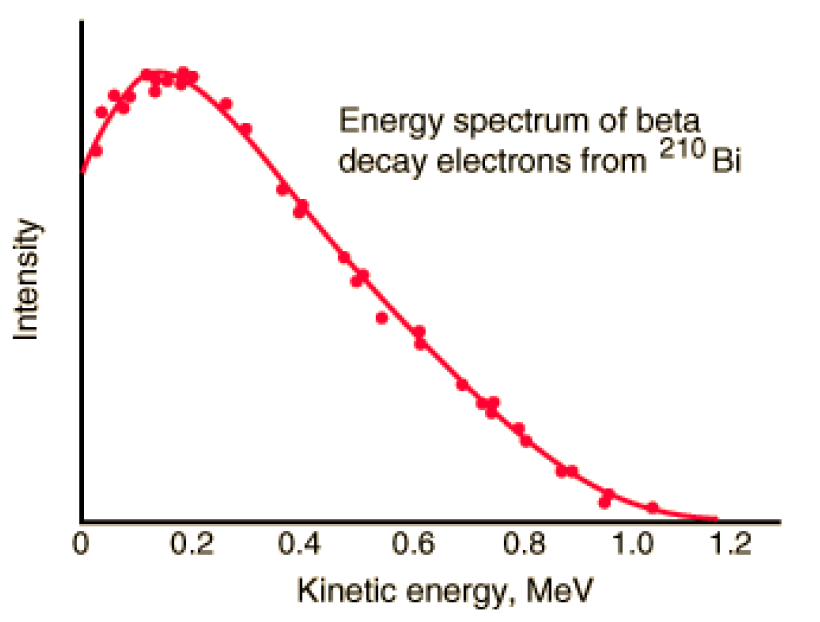
\includegraphics[width=7cm]{immagini/spettro_decadimento_beta_1.png}
   \end{figure}
\end{minipage}
\begin{minipage}{0.5\textwidth}
   \begin{figure}[H]
       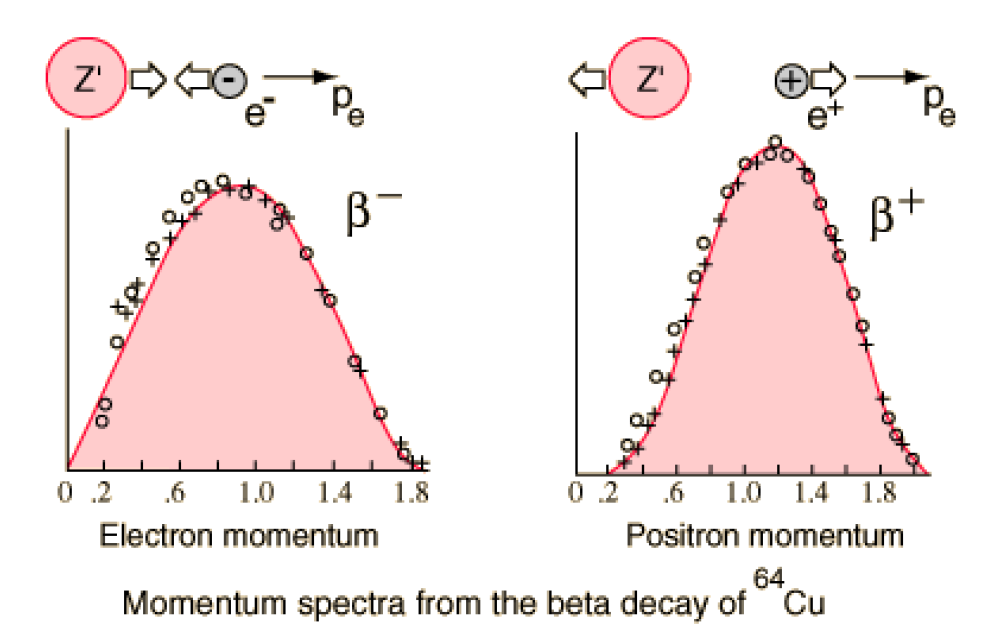
\includegraphics[width=9cm]{immagini/spettro_decadimento_beta_2.png}
   \end{figure}
\end{minipage}

\vspace{0.2cm}In realtà gli spettri dei decadimenti $\beta^+$ e $\beta^-$ sono leggermente diversi tra di loro a causa della repulsione coulombiana presente tra il nucleo residuo e l'elettrone/positrone. Ne segue che lo spettro del $\beta^+$ è shiftato a destra, cioè sono favoriti maggiormente degli impulsi (dunque delle energie) più grandi rispetto al $\beta^-$.

Ciò che è importante ricordare è che per questi elettroni ci aspettiamo energie che variano in maniera continua tra zero e un valore massimo.

%\subsection{Esempio: decadimento doppio \texorpdfstring{\ce{^{90}Sr / ^{90}Y}}{\textninesuperior\textzerosuperior Sr/\textninesuperior\textzerosuperior Y}}

\begin{esempio}[Decadimento doppio $^{\text{90}}$Sr/$^{\text{90}}$Y]
    Osserviamo lo spettro energetico del decadimento doppio \ce{^{90}Sr / ^{90}Y}:

    \begin{minipage}{0.7\textwidth}
        \begin{figure}[H]
            \centering
            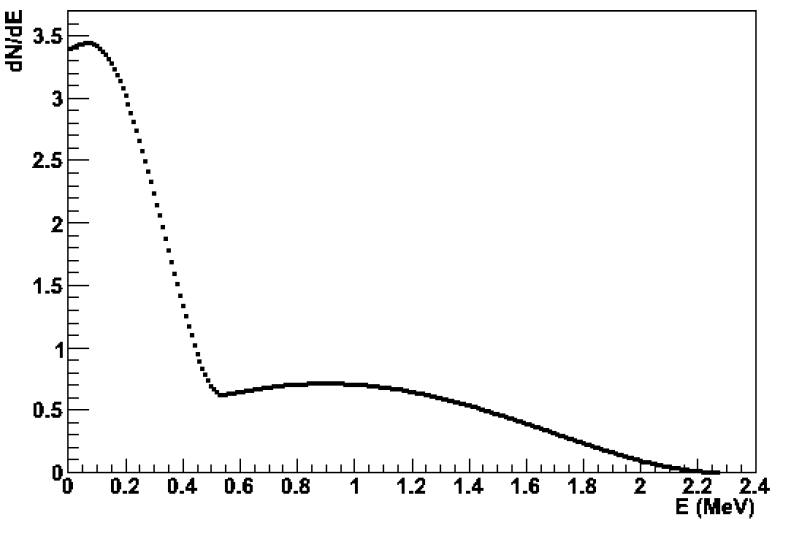
\includegraphics[width=9cm]{immagini/decadimento_beta_doppio.png}
        \end{figure}
    \end{minipage}
    \begin{minipage}{0.3\textwidth}

        \ce{^{90}Sr -> ^{90}Y} $(\beta^-)$

        \vspace{0.2cm}Vita media: 27.7 anni

        \vspace{0.2cm}$E_{\rm max}=0.546 \; \rm MeV$

        \vspace{0.8cm}\ce{^{90}Y -> ^{90}Zr} $(\beta^-)$

        \vspace{0.2cm}Vita media: 64 ore

        \vspace{0.2cm}$E_{\rm max}=2.27 \; \rm MeV$
    \end{minipage}

    \vspace{0.2cm}Essi sono decadimenti consequenziali, cioè lo stronzio-90 decade in ittrio-90 e quest'ultimo a sua volta decade ulteriormente.

    Lo spettro complessivo tiene conto di entrambi i decadimenti. In particolare la parte di basse energie corrisponde al decadimento dello stronzio, quella a più alta energia al decadimento dell'ittrio. Lo spettro finale, ricavabile dalla teoria di Fermi, è dato dalla sovrapposizione dei due spettri dovuti ai due isotopi. Si evince che abbiamo una grossa componente di elettroni a bassa energia ma anche una componente a più alta energia, fino ad un endpoint di circa 2.3 MeV.

    Andando a studiare i meccanismi di interazione degli elettroni con la materia, cioè come gli elettroni perdono energia, è possibile stimare lo spessore di materia necessario per fermare tutti gli elettroni emessi da questo tipo di sorgente.
\end{esempio}

\section[Isotopi radioattivi \texorpdfstring{$\alpha$}{\textalpha}]
{Isotopi radioattivi $\boldsymbol{\alpha}$}

\vspace{-0.6cm}\begin{figure}[H]
    \centering
    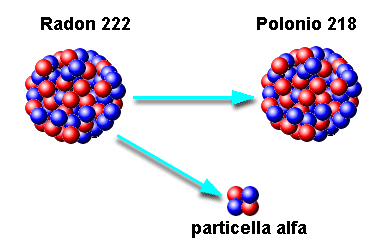
\includegraphics[width=8cm]{immagini/decadimento_alfa.png}
\end{figure}

\vspace{-0.2cm}Il decadimento $\alpha$ corrisponde all'emissione di una particella $\alpha$, che non è altro che un nucleo di elio ovvero costituito due protoni e due neutroni. Esso avviene nei nuclei pesanti. Osserviamo adesso uno schema di decadimento:

\begin{figure}[H]
    \centering
    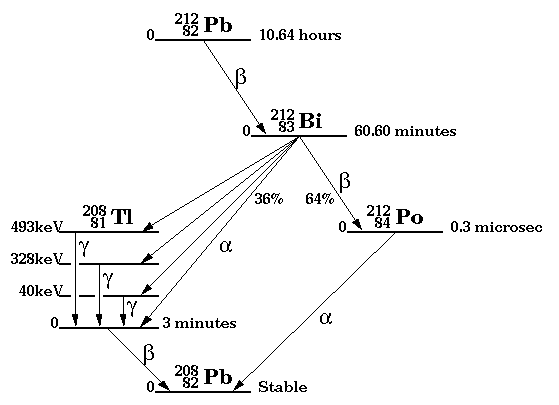
\includegraphics[width=11cm]{immagini/schema_decadimento_alfa.png}
\end{figure}

\vspace{-0.5cm}In esso ogni livello rappresenta un livello nucleare di un isotopo a una data energia. Si nota che si possono avere diversi decadimenti $\alpha$ verso lo stesso isotopo figlio, quello che cambia sono i livelli di energia di questo, per cui si può avere un decadimento verso un livello eccitato dell'isotopo figlio. Ognuno dei possibili decadimenti ha una sua probabilità di avvenire, detta \textit{branching ratio} (rapporto di ramificazione), quindi ci saranno decadimenti verso alcuni livelli più probabili rispetto a quelli verso altri livelli. Se il decadimento $\alpha$ avviene verso un livello eccitato, esso sarà inevitabilmente seguito da un decadimento $\gamma$, perché il nucleo, che si trova in uno stato eccitato, tenderà a portarsi nello stato fondamentale attraverso un decadimento $\gamma$. Va quindi ricordato che le particelle $\alpha$ emesse da un isotopo potrebbero avere energie diverse perché il decadimento può avvenire verso diversi livelli eccitati dell'isotopo figlio.

\vspace{0.2cm}Cosa ci aspettiamo in questo caso per lo spettro?

Essendo il decadimento $\alpha$ a due corpi (nucleo residuo e particella $\alpha$), tutta l'energia disponibile viene acquistata dalla particella $\alpha$ sotto forma di energia cinetica, in quanto è più leggera rispetto al nucleo residuo. Ci aspettiamo quindi che la particella $\alpha$ abbia sempre la stessa energia, ecco perché si parla di sorgenti monoenergetiche:

\vspace{-0.5cm}\begin{figure}[H]
    \centering
    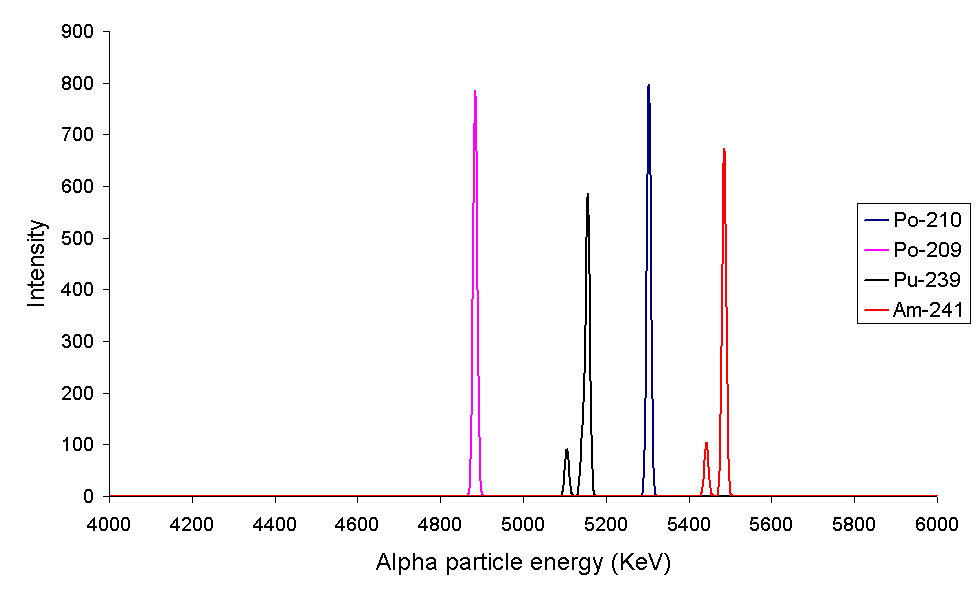
\includegraphics[width=11cm]{immagini/spettro_decadimento_alpha.png}
\end{figure}

\vspace{-0.5cm}Se misuriamo tale energia e la rappresentiamo in un istogramma otteniamo lo spettro energetico, che ci aspettiamo avere idealmente la struttura di una delta di Dirac, cioè dovremmo misurare sempre la stessa energia, come si vede in figura per vari isotopi. In realtà c'è una certa larghezza nel picco, che non è dovuta alla fisica di partenza (cioè le particelle $\alpha$ hanno veramente la stessa energia), bensì dipende dal modo con cui vengono misurate, dunque dalla precisione dello strumento di misura. L'allargamento del picco è quindi dovuto a questioni di risoluzione del rivelatore.

Vediamo alcuni esempi di isotopi che decadono $\alpha$:

\begin{center}
    \begin{tabular}{|l|l|l|}
        \hline
        Isotopo & Vita media & Alpha Energy (MeV)\\
        \hline
        &&\\[-0.45cm]
        $\rm ^{238}U$ & $4.5 \cdot 10^9$ y & $4.196/4.149$\\
        \hline
        &&\\[-0.45cm]
        $\rm ^{239}Pu$ & $2.4 \cdot 10^4$ y & $5.105/5.143/5.155$\\
        \hline
        &&\\[-0.45cm]
        $\rm ^{241}Am$ & 433 y & $5.443/5.486$\\
        \hline
    \end{tabular}
\end{center}

Notiamo che le energie delle particelle $\alpha$, nonostante le vite medie molto differenti, sono tutte molto simili, aggirandosi intorno a pochi MeV. La prima differenza tra radiazioni $\alpha$ e $\beta$ riguarda quindi lo spettro: le energie in gioco sono simili, ma lo spettro è molto diverso: continuo per le radiazioni $\beta$, "a righe" per le $\alpha$.

\section[Isotopi radioattivi \texorpdfstring{$\gamma$}{\textgamma}]
{Isotopi radioattivi $\boldsymbol{\gamma}$}

\vspace{-0.6cm}\begin{figure}[H]
    \centering
    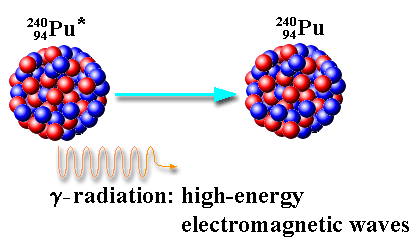
\includegraphics[width=8cm]{immagini/decadimento_gamma.png}
\end{figure}

\vspace{-0.4cm}In questo caso il decadimento avviene tra uno stato eccitato e uno stato a energia più bassa dello stesso nucleo, che quindi mantiene numero atomico e di massa invariato, mentre ciò che cambia è il suo livello energetico.

Nota: per indicare che un nucleo si trova nello stesso stato eccitato si usa un asterisco (Es. \ce{240^ Pu^*}).

Quando il nucleo passa allo stato fondamentale (cioè allo stato più basso in energia) emette una radiazione elettromagnetica che cade nella zona energetica dei $\gamma$.

Vediamo uno schema di livelli delle sorgenti (in laboratorio adopereremo \ce{^{60}Co} e \ce{^{137}Ce}):

\vspace{-0.4cm}\begin{minipage}{0.5\textwidth}
    \begin{figure}[H]
        \centering
        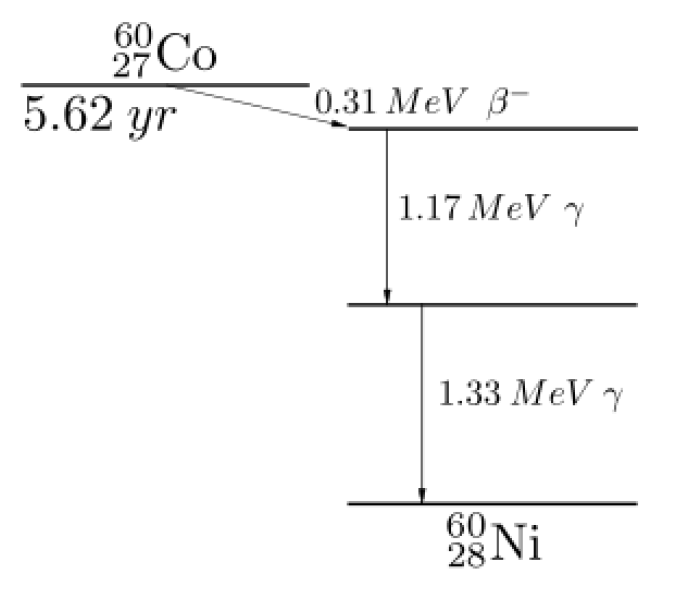
\includegraphics[width=7cm]{immagini/spettro_decadimento_gamma_1.png}
    \end{figure}
\end{minipage}
\begin{minipage}{0.5\textwidth}
    \begin{figure}[H]
        \centering
        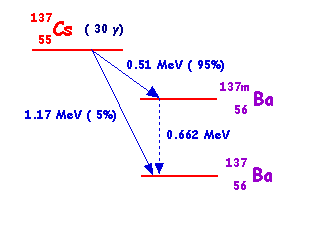
\includegraphics[width=8cm]{immagini/spettro_decadimento_gamma_2.png}
    \end{figure}
\end{minipage}

Notiamo come il \ce{^{60}Co} emette due $\gamma$ perché può avere diversi livelli nello stato finale, mentre il \ce{^{137}Ce} emette un solo $\gamma$.

\E interessante notare che il decadimento $\gamma$ è sempre consequenziale ad un'altra tipologia di decadimento (queste due sorgenti ad esempio decadono $\beta^-$).

\vspace{-0.2cm}

\begin{minipage}{0.495\textwidth}
    \begin{figure}[H]
        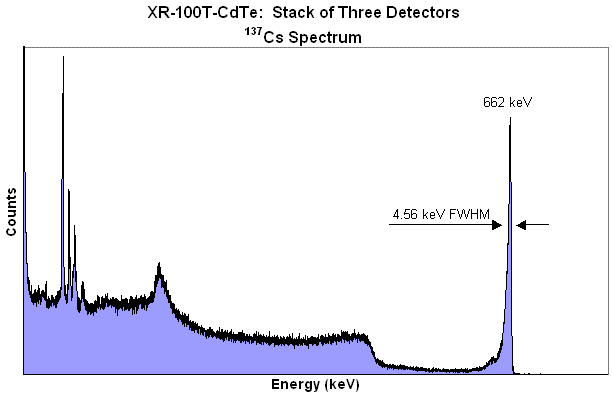
\includegraphics[width=7.5cm]{immagini/spettro_gamma.png}
    \end{figure}
\end{minipage}
\begin{minipage}{0.5\textwidth}
    \vspace{0.8cm}In termini di spettro energetico, anche in questo caso il gamma dovrebbe portare con sé tutta l'energia disponibile, quindi dovremmo avere uno spettro a righe. In realtà lo spettro misurato con un rivelatore ha una forma molto più complessa, per cui abbiamo un picco in corrispondenza del valore nominale di energia e poi un continuo per valori più bassi di energia (fondo continuo).
\end{minipage}

\vspace{0.2cm}Questo continuo lo spiegheremo in seguito, in quanto il $\gamma$ interagisce con il rivelatore attraverso diversi meccanismi che danno luogo a tale fondo continuo, tuttavia si osserva sempre un picco in corrispondenza dell'energia attesa.

I $\gamma$ sono quindi monoenergetici, ma anche qui ci possono essere effetti di risoluzione dell'apparato sperimentale che trasformano quella che dovrebbe essere una delta di Dirac in un picco con una data larghezza (tanto più largo è il picco, peggiore è la risoluzione, e se questa è scarsa nel caso del $\rm ^{60} Co$ c'è il rischio che i due picchi delle due emissioni si sovrappongano).

\section{Sorgenti di fissione}

Tra i fenomeni naturali si possono verificare anche delle fissioni. Alcuni nuclei pesanti possono, in maniera spontanea, frammentarsi in due nuclei di massa intermedia. Tale processo è detto di fissione. Ad esempio, l'$\rm ^{235}U$ in maniera spontanea si divide in $\rm ^{141}Ba$ e $\rm ^{92}Kr$. Oltre a questi due frammenti, si possono produrre anche dei neutroni, i quali a loro volta potrebbero innescare altri fenomeni di fissione (in questo caso si parla di fissione indotta). Tale meccanismo viene adoperato in maniera controllata dalle centrali nucleari, in quanto nel processo oltre ai frammenti di massa intermedia ed i neutroni viene prodotta anche energia; negli ordigni nucleari invece il processo di fissione indotta avviene fuori controllo.

Nella fissione i frammenti che vengono prodotti non sono mai simmetrici: ciò è dovuto a questioni di bilancio energetico nel processo di fissione.

\begin{minipage}{0.58\textwidth}
    \begin{figure}[H]
        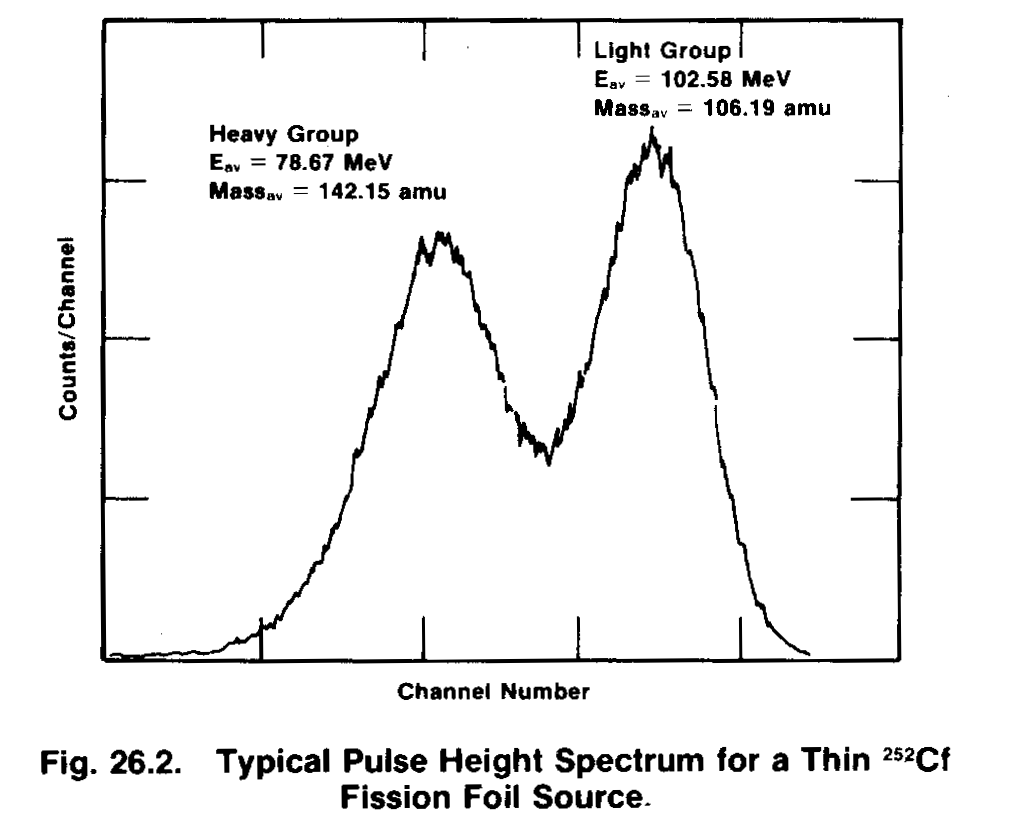
\includegraphics[width=9cm]{immagini/Sorgenti_di_fissione_1.png}
    \end{figure}
\end{minipage}
\begin{minipage}{0.42\textwidth}
    \begin{figure}[H]
        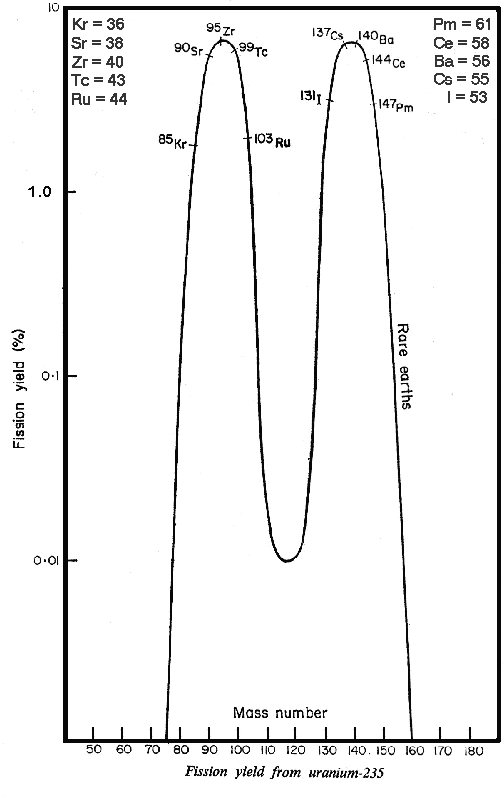
\includegraphics[width=6cm]{immagini/Sorgenti_di_fissione_2.png}
    \end{figure}
\end{minipage}

\vspace{0.3cm}Nel grafico a destra possiamo vedere la distribuzione del numero di massa dei frammenti. Essa ha una forma a due picchi, che indica il fatto che i frammenti non assumono valori di massa qualsiasi, bensì preferenzialmente assumono valori che si concentrano sui picchi. Tale asimmetria ha come conseguenza che anche le energie dei frammenti non sono esattamente le stesse: il frammento più leggero prenderà più energia e viceversa quello più pesante, come possiamo vedere nel grafico a sinistra raffigurante la distribuzione delle energie dei frammenti.

\section{Radiazione cosmica}

Negli alti strati dell'atmosfera i raggi cosmici primari incidono e interagiscono con gli atomi e le molecole dell'atmosfera, dando origine ai cosmici secondari.

I cosmici primari sono costituiti da protoni (anche nuclei però, perché la composizione di tali raggi rispecchia l'abbondanza dei diversi nuclei presenti nello spazio) aventi energia elevatissima, che interagendo con l'atmosfera generano cascate di particelle il cui numero è proporzionale all'energia del cosmico primario. Alcune di queste particelle compongono la parte elettromagnetica dello sciame (gamma, elettroni, positroni), altre la parte più penetrante, ad esempio i muoni.

\begin{minipage}{0.5\textwidth}
    \begin{figure}[H]
        \centering
        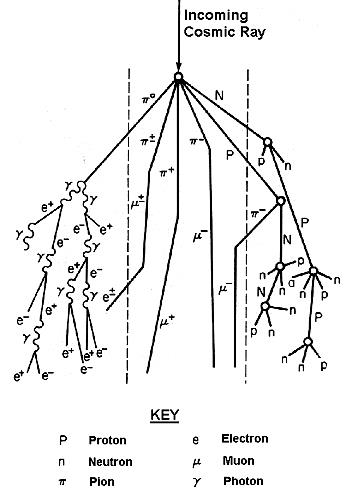
\includegraphics[width=7cm]{immagini/radiazione_cosmica.png}
    \end{figure}
\end{minipage}
\begin{minipage}{0.5\textwidth}
    \begin{figure}[H]
        \centering
        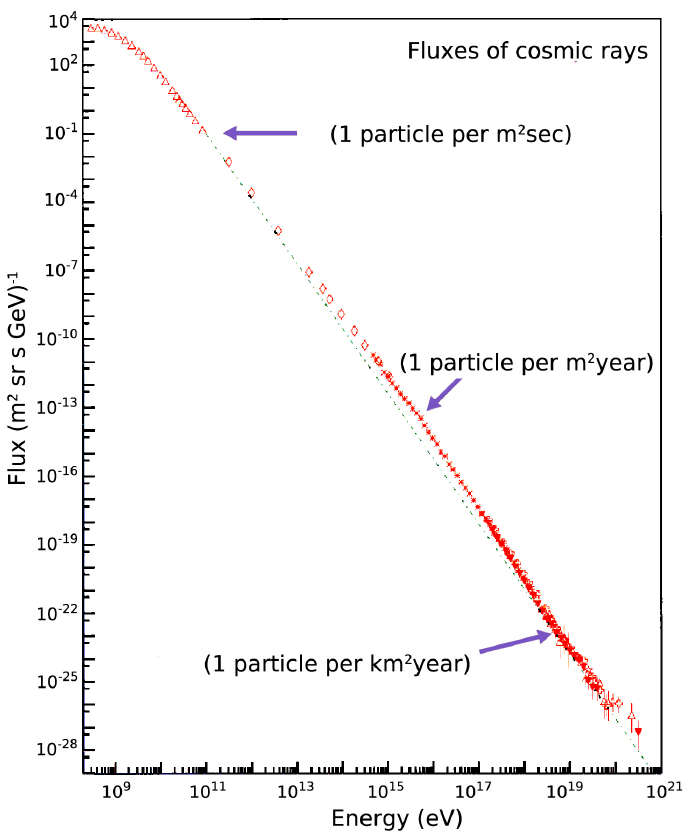
\includegraphics[width=8cm]{immagini/energia_radiazione_cosmica.png}
    \end{figure}
\end{minipage}

\vspace{0.4cm}Lo spettro di energia dei cosmici primari (rappresentato in scala logaritmica sia in ascisse che in ordinate perché ci sono numeri che variano parecchio) ha in ascisse l'energia, che varia da $10^9$ a $10^{21}$ eV, e in ordinata il flusso, cioè il numero di particelle che arrivano per metro quadro e nell'unità di tempo con una data energia, che varia da $10^{-28}$ a $10^4$. Tale grafico ci dice che ad esempio per valori di energia intorno a $10^{11}/10^{12}$ eV, avendo a disposizione di un rivelatore della superficie di 1 $\rm m^2$ misureremo circa una particella al secondo, mentre per i primari più energetici ($10^{20}$ eV) ci servirebbe un rivelatore di 1 $\rm km^2$ per misurare una particella per anno. Essendo quest'ultime molto rare, di solito si studiano i cosmici secondari e si cerca di ricostruire le energie dei primari (e in questo caso si parla di \textit{rivelazione indiretta}), mentre alle basse energie è possibile effettuare delle misure dirette portando un rivelatore al di fuori dell'atmosfera terrestre e misurando il flusso di raggi cosmici.

\section{Unità di misura e nomenclatura}

\subsection{Attività di una sorgente}

Rappresenta il numero di particelle emesse nell'unità di tempo. Si misura in

\begin{itemize}
    \item Becquerel (Bq): $\rm 1 \; Bq=1 \; disintegrazione/s$;
    \item Curie (Ci): $\rm 1 \; Ci=3.7 \cdot 10^{10} \; disintegrazioni/s$ (attività di 1 g di $\ce{^{226}Ra}$). Esprime una grandezza molto grande, per cui si preferisce lavorare con sottomultipli come il $\rm \mu Ci$. Si ha che $\rm \mu Ci=37 \cdot 10^3 \; Bq$.
\end{itemize}

\subsection{Concetto di dose}
La dose rappresenta l'energia che viene depositata da una radiazione per unità di massa. Si misura in $\rm J/kg$, quantità che viene chiamata Gray (Gy). $\rm 1 \; Gy$ corrisponde a $\rm 1 \; J/1 \; kg$. Alternativamente si può adoperare il rad, unità di misura tale che $\rm 1 \; Gy=100 \; rad$.

\subsection{Concetto di dose equivalente}
Tale concetto viene introdotto perché non è importante soltanto quanta energia viene depositata per unità di massa, ma anche il tipo di radiazione che ha depositato quell'energia, informazione che ci aiuta a capire il danno prodotto da una radiazione ad esempio nell'organismo.

La dose equivalente è pari alla dose moltiplicata per un fattore di qualità, il quale dipende dal tipo di radiazione: esso vale
\begin{itemize}
    \item $\sim 1$ per gamma e beta;
    \item $\sim 10$ per protoni e neutroni veloci;
    \item $\sim 20$ per alfa.
\end{itemize}
Deduciamo che, a parità di energia depositata per unità di massa, sono più dannose le particelle alfa; a seguire i protoni e ancora dopo i gamma. \E chiaro che il danno dipende anche dal tessuto colpito.

La dose equivalente si misura in Sievert (Sv) o rem.

$\rm 1 \; Sv=(\text{Fattore di qualità}) \cdot 1 \; Gy$
$\rm 1 \; Sv=100 \; rem \quad 1 \; mSv=100 \; mrem$

\subsection{Dosi tipiche}

Vediamo a che livello di radiazioni siamo sottoposti quotidianamente.

\subsubsection{Sorgenti naturali}

\begin{itemize}
    \item Radiazione cosmica: 28 $\rm mrem/anno$;
    \item Fondo naturale (isotopi naturali): 26 $\rm mrem/anno$;
    \item Radioattività interna al corpo\footnotemark: 26 $\rm mrem/anno$;
\end{itemize}

\footnotetext{Noi emettiamo $\beta$ a causa del $\rm ^{14}C$ e del $\rm ^{40}K$.}

\subsubsection{Sorgenti artificiali}

\begin{itemize}
    \item Radiografia: variabile a seconda del tipo. Ad esempio una RX al torace corrisponde a qualche $\rm mrem$, una TAC a $10^3 \; \rm mrem$.
\end{itemize}

\E chiaro che ci sono dei limiti che bisogna rispettare affinché si eviti il danno biologico. Tale limite è variabile (a seconda che sia una persona qualunque o un lavoratore esposto). In genere per la popolazione il limite è $200 - 300$ mrem/anno.

Ci sono poi delle condizioni in cui siamo esposti, in maniera naturale, ad una maggiore dose di radiazioni. Ad esempio in alta montagna (a quote di $2000-3000$ m) si è esposti ad una maggiore radiazione perché viene meno il "filtro" dell'atmosfera.

\subsubsection{Trivia: il caso della banana}

Proviamo a stimare l'attività dovuta a un certo quantitativo di banane, in maniera tale da capire se sono dannose.

In media una banana contiene 0,5 g di $\rm ^{40}K$, che corrisponde a un'attività di $\rm 15 \; Bq=15 \; disintegrazioni/secondo$. A causa della loro diffusione, è stata creata la dose dovuta al mangiare una banana: 1 BED (\textit{Banana Equivalent Dose}) $\sim 0,1 \; \rm \mu Sv$. Ogni giorno siamo sottoposti a una dose di radiazione naturale di 100 BED; una radiografia corrisponde a $5 \cdot 10^4$ BED. QUesti esempi ci fanno capire come una banana non sia affatto dannosa.